\documentclass[12pt]{article}
\usepackage{setspace}   % paquete para interlineado
\usepackage{newtxtext,newtxmath} % Times New Roman

%otra opcion para times roman adaptable a versiones
%\usepackage{mathptmx}

%haber si funciona mas parecido a word
\setstretch{1.5}  
%\usepackage[protrusion,expansion]{microtype}
%\onehalfspacing               % interlineado 1.5
\usepackage{amsmath} % Para usar \text{}
\usepackage[utf8]{inputenc}
\usepackage[spanish]{babel}
\usepackage[letterpaper, left=3cm, right=2.5cm, top=2.5cm, bottom=2.5cm]{geometry}
\usepackage{graphicx}
\usepackage{titlesec}
\usepackage{setspace}
\usepackage{lipsum}
\geometry{margin=1in}


%PAQUETE para incluir PDF´s
\usepackage{pdfpages} % para incluir PDFs

% ---PAQUETE PARA contador para las introducciones ---
\newcounter{intro}
\renewcommand{\theintro}{\arabic{intro}} % numeración arábiga: 1,2,3,...


% PAQUETE PARA COMENTAR FACILMENTE 

\usepackage{comment}

%%FORZAR LAS IMAGENES CON FLOAT

\usepackage{float} % necesario para usar [H]


% ESPACION DE TITULOS*{comando}{margen_izq}{espacio_antes}{espacio_despues}
%\titlespacing*{\section}
%{0pt}    % sangría izquierda
%{3em}    % espacio ANTES del título
%{0em}    % espacio después del título




 % PAQUETE PARA INSTANCIAR  LAS IMAGENES
  \graphicspath{{./Imagenes}}
 

%CONFIGURACION DE MI PAGINA numeración:
%\usepackage{fancyhdr}
%\pagestyle{fancy}
%\fancyhf{} % Limpia encabezados/pies
%\fancyhead[R]{\thepage} % Números arábigos arriba: izq en pares, der en impares
%\renewcommand{\headrulewidth}{0pt} % Sin línea

%COLOCAR NUMERACION ESQUINA DERECHA PAG 1
%\fancypagestyle{plain}{%
%	\fancyhf{}%
%	\fancyhead[R]{\thepage}%
%	\renewcommand{\headrulewidth}{0pt}%



% --- PAQUETES ADICIONALES DE LOSA ---
  % para listas multinivel (numeración + incisos + viñetas)
\usepackage{enumitem} 

% que los párrafos  de las secciones dentro de los items usen la misma sangría que el cuerpo SANGRIA A TODOWWW
\setlist[enumerate]{listparindent=\parindent, parsep=0pt}

\begin{comment}
	
	% --- Configuración de enumitem para numeración multinivel ---
	\setlist[enumerate,1]{label=\arabic*., leftmargin=1.2cm}
	\setlist[enumerate,2]{label=\arabic{enumi}.\arabic*., leftmargin=1.4cm}
	\setlist[enumerate,3]{label=\arabic{enumi}.\arabic{enumii}.\arabic*., leftmargin=1.6cm}
	\setlist[enumerate,4]{label=\alph*) , leftmargin=1.8cm}
	\setlist[itemize]{leftmargin=1.6cm}
	
\end{comment}


\begin{comment}
	PARA INDICES CREO
	\tableofcontents
	\newpage
\end{comment}



\begin{document}
	
	%Para no generar numeracion de paginas
	\pagestyle{empty}
	
%	\thispagestyle{fancy} 
	
	%es para emparejar el tamaño de todas las letras de titulo y contenido
%	\titleformat{\section}{\large\bfseries}{\thesection.}{0.5em}{}
%	\titleformat{\subsection}{\normalsize\bfseries}{\thesubsection.}{0.5em}{}
	
	%\title{\vspace{-2cm}Área de Métodos Constructivos
%	\\ Descripción y proceso constructivo de losas}
%	\author{}
%	\date{}
	

	
	
	
%	\maketitle
	
	%\vspace{-2.5cm}
	
%
\includepdf{portadaU2/caratulaU}
%
\includepdf[pages=-,pagecommand={}]{hoja/hojaadjunta}

%%-----------TITULOSSSS--------------------------------------
		\begin{center}
		\textbf{\LARGE Área de Métodos constructivos}
	\end{center}

%--------------SUBTITULOS---------------------

	% Primera introducción
\stepcounter{intro}
\section*{\theintro\ Descripción y proceso constructivo de losas}
\addcontentsline{toc}{section}{\theintro\ Descripción y proceso constructivo de losas}
 

	
%-------------LOSA TRADICIONAAAAL--------------------




	\section{Losa Tradicional}

La losa tradicional, también llamada losa maciza, es un elemento estructural sólido de concreto reforzado, soportado por vigas o muros, con espesor uniforme en toda su extensión. Se utiliza de manera frecuente en edificios residenciales, comerciales e industriales, así como en obras donde se presentan cargas concentradas importantes que requieren alta rigidez y continuidad estructural.

El proceso constructivo de este tipo de losa constituye una de las actividades más relevantes dentro de la ejecución de estructuras de concreto en Guatemala. Su correcta ejecución no solo depende de la experiencia de la mano de obra, sino también del cumplimiento de normas y códigos técnicos que establecen criterios de diseño, recubrimientos, tolerancias y tiempos adecuados de curado y desencofrado. Entre ellos destacan la Norma Sísmica de Edificación NSE 7.1 (que adopta el ACI 318S-19), la guía ACI 347R para encofrados y la ACI 308R sobre curado del concreto, además de normas guatemaltecas como la NTG 41068 para concreto premezclado.

En este sentido, el proceso constructivo de una losa tradicional maciza incluye fases claramente definidas: preparación del sitio, montaje del encofrado y apuntalamiento,  del acero de refuerzo, vaciado del concreto, curado y desencofrado. El cumplimiento ordenado y riguroso de cada etapa asegura que la losa alcance la resistencia, durabilidad y seguridad estructural necesarias, garantizando su adecuado desempeño como diafragma rígido y elemento portante dentro de la edificación.

%\vspace{0.5} % agrega 1 cm de espacio
\begin{figure}[h]
	\centering
	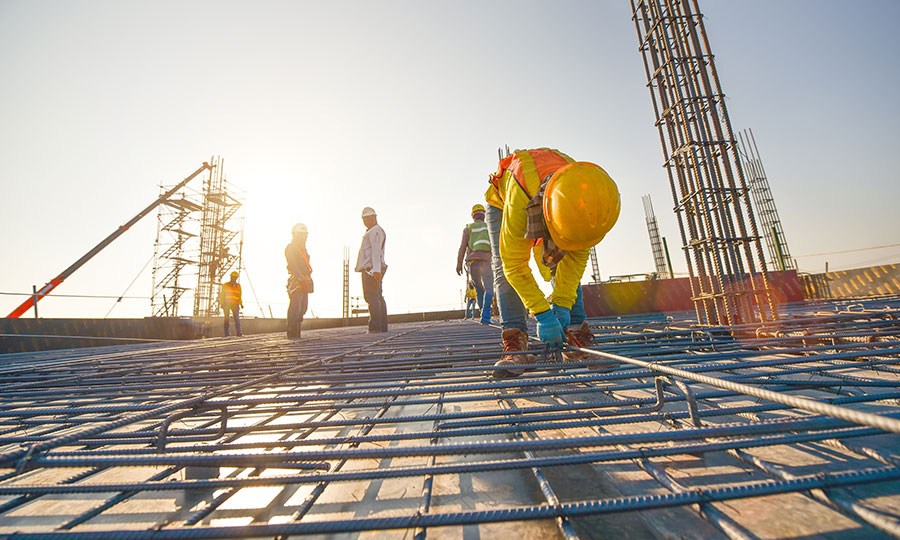
\includegraphics[width=0.6\textwidth]{losa1}
	\caption{Proceso de armado con retícula y refuerzos perimetrales}
	\label{fig:losa1}
\end{figure}

	\subsection{Preparación y limpieza del sitio}
	Se debe tener un ambiente de trabajo limpio y libre de obstáculos, en el que se
	puedan movilizar libremente las personas y maquinarias que participarán en la
	obra. Este paso incluye la deforestación y remoción de cualquier capa vegetal que
	pudiera entorpecer el trabajo, la limpieza y explanación del terreno en caso de
	tratarse de una losa de fundación o la losa de la planta baja. Procesos a considerar:
	\begin{enumerate}
		\item Retirar escombros, basura y obstáculos del área de trabajo.
		\item Nivelar y trazar el perímetro conforme a planos estructurales.
		\item Preparar accesos para el traslado de materiales y equipos.
	\end{enumerate}
	
	%\vspace{0.5} % agrega 1 cm de espacio
	\begin{figure}[h]
		\centering
		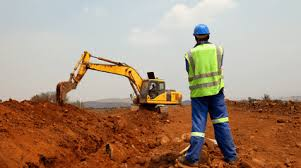
\includegraphics[width=0.6\textwidth]{losa2}
			\caption{Limpieza de terreno}
		\label{fig:losa2}
	\end{figure}
	
	%-----------------------------
	
	\subsection{Preparación de Materiales y herramientas}
	Al momento de iniciarse la obra se deben contar con todos los implementos que
	se van a necesitar al igual que tener todos los materiales a disposición para que el
	proceso no se vea interrumpido o paralizado por la falta de alguno de los
	anteriores.
	
	Como se observa en la figura 3, se encuentran elementos como materiales, maquinarias y herramientas
	necesarias para la jornada planificada. En el fondo la arena y la piedra picada, a la
	derecha las cabillas y la malla electrosoldada. Puntales de acero, madera para
	encofrado, mezcladora de concreto, etc.
	
	
	
	\begin{enumerate}
		\item \textbf{Herramientas}
		\begin{enumerate}[label=\alph*)]
			\item Serrucho, martillo, escuadra, plomada, nivel, cinta métrica.
			\item Palas, picos, carretillas y regletas metálicas.
			\item Ganchos para amarre y dobladora de varilla.
		\end{enumerate}
		\item \textbf{Equipos}
		\begin{enumerate}[label=\alph*)]
			\item Mezcladora, vibrador de aguja, andamios y escaleras.
			\item Sistemas de izaje o bombas de concreto en niveles superiores.
		\end{enumerate}
		\item \textbf{Materiales}
		\begin{enumerate}[label=\alph*)]
			\item Cemento Portland, arena, grava y agua potable.
			\item Acero de refuerzo y malla electrosoldada.
			\item Tuberías PVC para instalaciones eléctricas e hidrosanitarias.
			\item Madera o formaletas metálicas y desmoldante.
		\end{enumerate}
	\end{enumerate}
	
	\begin{figure}[h!]
		\centering
		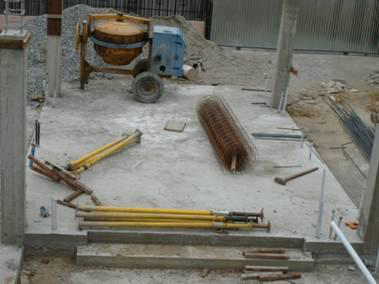
\includegraphics[width=0.6\textwidth]{losa3}
		\caption{Materiales y herramientas}
		\label{fig:losa3}
	\end{figure}
	
	%---------------------------------
	
	
	\subsection{Encofrado y apuntalamiento}

	El encofrado es la \textit{estructura temporal} que da forma al concreto fresco, soporta su peso y mantiene en posición el refuerzo hasta que la mezcla alcance resistencia.
	
	Su función principal es ofrecer la posibilidad de que el acero de refuerzo
	sea colocado en el sitio correcto, darle al concreto la forma y servirle de apoyo
	hasta que endurezca, está constituido por el molde y los puntales, que pueden ser
	metálicos o de madera. Existen una gran cantidad de tipos de encofrado, de distintos materiales y de
	distintas formas, cada uno es utilizado para un fin específico
	
	\subsubsection{Tipos de encofrado}
	
	\begin{enumerate}
		\item \textbf{Madera}
		
		Presentan la ventaja de que pueden ser cortados para
		darles la forma deseada, sin embargo esto genera desperdicios de material que en
		ocasiones no se puede reutilizar. Para alargar la vida útil del encofrado y que se
		pueda reutilizar en distintas obras se le debe dar un cuidado especial como se
		indica:
		
		\begin{enumerate}[label=\alph*)]
			\item Fácil de cortar y adaptar a diferentes geometrías.
			\item Debe limpiarse y almacenarse protegido para prolongar su vida útil.
			\item Aplicar desmoldante para facilitar el desencofrado.
		\end{enumerate}
		\item \textbf{Metálico}
	
		Los encofrados metálicos presentan un desgaste mínimo con un manejo
		adecuado. Al igual que los de madera deben ser tratados de manera especial:
		
		
		\begin{enumerate}[label=\alph*)]
			\item 
			Se deben limpiar bien luego de usarlos, e impregnarlos con un producto
			desmoldante comercial: aceite, petróleo o gasoil con parafina al 50%,
			dependiendo del acabado que se quiera lograr.
			\item 
			Se debe evitar la oxidación protegiéndolos periódicamente con pintura
			anticorrosiva, sobre todo si van a estar mucho tiempo a la intemperie.
			
			\item 
			Debe protegérsele también de los rayos del sol y de la lluvia.
			
			\item 
			Se debe almacenar en sitios cubiertos y secos, debidamente codificados,
			colocado verticalmente o ligeramente inclinado cuando se recuesten sobre
			un muro y levantados del piso sobre zancos o tacos.
			
		\end{enumerate}
		
		
		\item \textbf{Plástico (casetones)}
		
		Son los más usados para el vaciado de losas nervadas y
		reticulares ya que vienen con formas y dimensiones predefinidas para tal fin. Su
		principal ventaja es que son muy fáciles de manipular y colocar en sitio debido a
		su ligereza
		
		\begin{enumerate}[label=\alph*)]
			\item Usados en losas nervadas o reticulares.
			\item Ligeros y de fácil manipulación, aunque delicados.
		\end{enumerate}
	\end{enumerate}
	
	
	\begin{figure}[h]
		\centering
		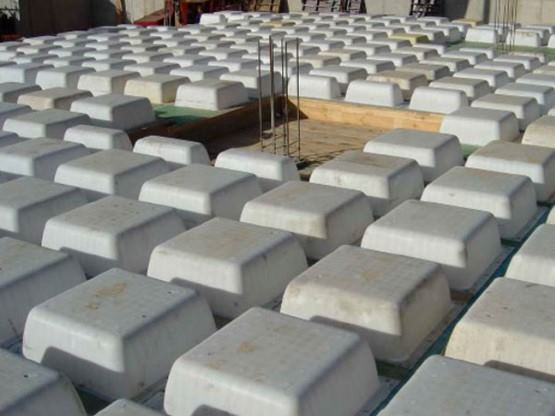
\includegraphics[width=0.7\textwidth]{losa4}
		\caption{Sistema de casetones recuperable}
		\label{fig:losa4}
	\end{figure}
	
	
	
	\subsubsection{Puntales}
	
	Los puntales los elementos que le proporcionan soporte al encofrado hasta
	que el concreto fragüe y la estructura sea capaz de resistir las cargas debidas a su
	propio peso
	
	\begin{enumerate}
		\item Los puntales pueden ser de madera o metálicos telescópicos.
		\item Deben colocarse plomados, sobre bases firmes y arriostrados.
		\item Su función es resistir el peso del concreto fresco y cargas de construcción.
	\end{enumerate}
	

	\begin{figure}[h]
	\centering
	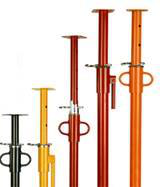
\includegraphics[width=0.35\textwidth]{losa5}
	\caption{Puntales Metálicos}
	\label{fig:losa5}
\end{figure}

	
	\subsection{Colocación del acero de refuerzo Inferior}
	Luego de haber encofrado y apuntalado correctamente la losa se procede a la
	colocación del acero de refuerzo de la misma. Es evidente que previamente se
	debió haber cortado y doblado las cabillas de acuerdo a los planos del despiece.
	Es importante que las barras se fijen firmemente en su posición para evitar que se
	muevan cuando se esté vaciando el concreto, también debemos respetar los
	recubrimientos que deben tener, si es necesario se pueden apoyar sobre tacos de
	concreto que tengan una altura igual a la del recubrimiento y una resistencia
	mayor o igual a la del concreto que se vaciará en la losa.
	
	
	\subsection{Colocación de las tuberías y conductos para
		instalaciones eléctricas e hidrosanitarias}
		
		De acuerdo al uso de la edificación o del nivel que se esté por construir, se puede
		decidir entre embutir las tuberías y conductos en la losa o si colgarlos para que
		vayan debajo de la misma, quedando a la vista desde el nivel inferior. De cualquier
		manera se deben ubicar en su posición antes de vaciar el concreto. En el caso de
		las tuberías destinadas a las instalaciones eléctricas se recomienda pintarlas o
		etiquetarlas de manera que se puedan distinguir entre las tuberías de apagadores,
		tomacorrientes, etc.
		
	\begin{enumerate}
		\item Instalar tuberías eléctricas e hidrosanitarias antes del vaciado.
		\item Sujetar firmemente para impedir movimiento.
		\item Etiquetar tuberías eléctricas para identificación.
	\end{enumerate}
	
	\subsection{Colocación del acero de refuerzo superior}
	Se coloca el acero superior teniendo las mismas precauciones que el acero
	inferior. Si no se requiere de la colocación de barras de refuerzo se coloca la malla
	electrosoldada de acuerdo a los planos de despiece.
	
	\begin{enumerate}
		\item Colocar varillas o malla electrosoldada en la parte superior.
		\item Respetar los recubrimientos mínimos.
	\end{enumerate}
	

	\subsection{Vaciado del concreto}
	Luego de tener todos los elementos de la losa ubicados en su sitio, se lleva a cabo
	el proceso de vaciado de concreto, el cual puede ser mezclado en obra o traído de
	una planta de premezclado.
	El vaciado se puede realizar con la utilización de herramientas simples como
	baldes y carretillas si se trata de la planta baja o los niveles inferiores de la
	edificación (máximo hasta el segundo nivel) con la ayuda de un sistema de poleas.
	Para niveles superiores se puede realizar con la utilización de una grúa y un
	carretón, o mediante la utilización de bombas que lleven el concreto a través de
	tuberías.
	
	\subsubsection{Procedimiento}
	\begin{enumerate}
		\item Transportar el concreto en carretillas, baldes o mediante bomba.
		\item Descargar en capas uniformes para evitar segregación.
		\item Vibrar con aguja para compactar y eliminar vacíos.
		\item Nivelar con reglas metálicas y palustre.
	\end{enumerate}
	
	
	\subsection{Curado de concreto}
	El objetivo principal del curado es el de evitar que se evapore el agua de la
	mezcla, lo que podría producir grietas de retracción debido a la pérdida de
	humedad y alteraciones en la relación agua/cemento de la mezcla, lo que incide
	directamente en su resistencia. Para obtener mejores resultados, se recomienda
	humedecer el concreto durante los primeros 7 días de vaciado.
	El proceso del curado empieza incluso antes del vaciado del concreto, al mantener
	humectado el encofrado, para así evitar la pérdida del agua por la absorción de la
	madera.
	
	\subsubsection{Métodos}
	\begin{enumerate}
		\item Mantener la superficie húmeda al menos durante 7 días.
		\item Aplicar riego frecuente o cubrir con plásticos/membranas.
		\item En climas cálidos: regar más seguido y proteger con sacos mojados.
		\item En climas fríos: prolongar el curado por el fraguado lento.
	\end{enumerate}
	

	
	\subsection{Desencofrado y desapuntalamiento}
	Una vez iniciado el fraguado del concreto se pueden comenzar a retirar los
	encofrados laterales de la losa y posteriormente se pueden retirar algunos
	puntales. El desapuntalamiento se debe ir haciendo en forma progresiva a medida
	que van pasando los días, hasta que se pueden retirar todos los puntales y el
	encofrado a los 21 días.
	
	\subsubsection{Criterios}
	\begin{enumerate}
		\item Retirar primero las formaletas laterales.
	%	\item Quitar los puntales en forma progresiva tras alcanzar la resistencia mínima (≈70\% f’c).
		\item Completar el desapuntalamiento a los 21 días, salvo indicación distinta en planos.
	\end{enumerate}
	

	
	
	
	%-----------------------------------------------------------
	

	
		
	%----------VIGUETA Y BOVEDILLA-------------------------------
	
	\section{Vigueta y Bovedilla}
	

	Es un sistema de \textbf{losa prefabricada unidireccional} compuesto por \textbf{viguetas} (prefabricadas de concreto armado o presforzado), \textbf{bovedillas} (elementos de relleno: concreto ligero, arcilla, EPS, etc.), y una \textbf{capa de compresión} de concreto colada en sitio. Suele incluir \textbf{malla de refuerzo} superior y \textbf{rigidizantes} transversales (nervios de amarre). La norma guatemalteca \textbf{NTG 41084} define el sistema, componentes, criterios de aceptación, manejo y el concepto de \textit{rigidizante} (nervio transversal), entre otros.
	
	
	\begin{figure}[h]
		\centering
		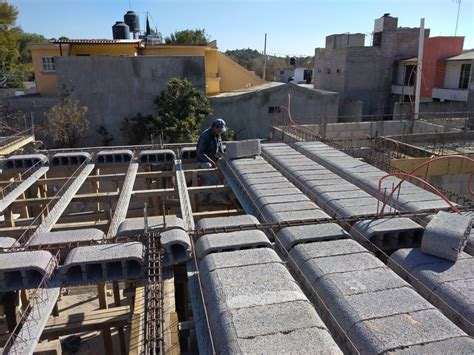
\includegraphics[width=0.7\textwidth]{vigueta_bovedilla_esquema_real.png}
		\caption{Vista general del sistema vigueta--bovedilla en obra.}
		\label{fig:vigueta_bovedilla_esquema_real}
	\end{figure}
	
	\subsection{Marcos normativos clave (Guatemala y ACI)}
	\begin{itemize}
		\item \textbf{AGIES / NSE (Guatemala):}
		\begin{itemize}
			\item \textbf{NSE 7.1 – Concreto estructural}: requisitos de diseño y construcción (armado, recubrimientos, tolerancias, etc.).
			\item \textbf{NSE 7.3 – Elementos prefabricados y preesforzados}: aplica cuando las viguetas son prefabricadas/presforzadas y armoniza con ACI 318.
			\item \textbf{NSE 3 – Diseño estructural de edificaciones (ed. 2024)}: norma marco que remite a NSE 7.1 y 7.3 según el sistema.
			\item \textbf{NTG 41084}: requisitos mínimos para viguetas y bovedillas, definiciones, almacenamiento, transporte, criterios de aceptación en obra y rigidizantes.
		\end{itemize}
		\item \textbf{ACI (Estados Unidos):}
		\begin{itemize}
			\item \textbf{ACI 318}: reglas de diseño para sistemas de viguetas/joists y losas unidireccionales, controles de flecha (espesores mínimos o cálculo de deflexiones), cuantías y detallado de refuerzo.
			\item \textbf{ACI 308R}: prácticas estándar de curado del concreto, métodos y duraciones.
		\end{itemize}
	\end{itemize}
	
	\textbf{Regla general de aplicación}: en Guatemala diseñas/ejecutes con \textbf{NSE/AGIES} y \textbf{NTG 41084}; donde éstas remiten o guardan silencio, aplicas \textbf{ACI 318} (diseño/constructivo) y \textbf{ACI 308R} (curado).
	
	\subsection{Proceso constructivo}
	
	\subsubsection{ Planeación y recepción en obra}
	\begin{enumerate}
		\item \textbf{Revisión de planos y memoria}: confirmar cargas, luces, dirección de las viguetas, posición de rigidizantes y cuantía de capa de compresión y malla.
		\item \textbf{Recepción de prefabricados}: verificar que viguetas y bovedillas cumplan NTG 41084 (marcado, dimensiones, integridad, resistencia declarada). Registrar criterios de aceptación y rechazo de piezas dañadas.
		\item \textbf{Almacenamiento y manejo}: apilar en superficie plana, con durmientes alineados; proteger bovedillas frágiles; seguir indicaciones de NTG 41084 para transporte y almacenamiento.
	\end{enumerate}
	
	\begin{figure}[h]
		\centering
		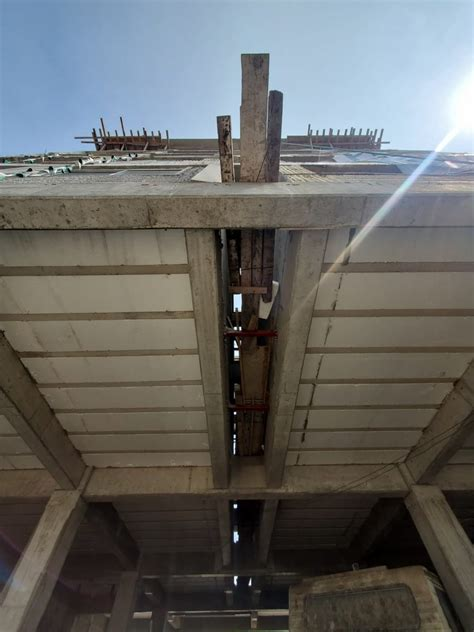
\includegraphics[width=0.5\textwidth]{recepcion_material.png}
		\caption{Recepción y verificación de piezas (viguetas y bovedillas).}
		\label{fig:recepcion_material}
	\end{figure}
	
	\subsubsection{ Preparación de apoyos y apuntalamiento}
	\begin{enumerate}
		\item[4.] \textbf{Apoyos}: verificar nivelación de vigas/muros de apoyo y recubrimientos; saturar superficialmente si corresponde.
		\item[5.] \textbf{Apuntalamiento}: trazar e instalar arriostrados según el plan del proveedor/ingeniero; respetar flechas de contra–flecha si están especificadas.
	\end{enumerate}
	
	\subsubsection{ Montaje de viguetas y bovedillas (armado e instalación)}
	\begin{enumerate}
		\item[6.] \textbf{Colocación de viguetas}: orientar en la dirección resistente; espaciar según planos/tablas del proveedor; apoyos mínimos definidos por NTG/planos; revisar alineación.
		\item[7.] \textbf{Colocación de bovedillas}: insertar entre viguetas sin golpear; completar paños; prever pasos para instalaciones sin debilitar nervios.
		\item[8.] \textbf{Rigidez transversal (rigidizantes)}: ejecutar nervios transversales donde indique el diseño para controlar torsión y diafragma.
		\item[9.] \textbf{Refuerzo superior}: colocar malla electrosoldada o varillas en la capa de compresión; colocar aceros negativos sobre apoyos, ganchos y traslapes según NSE 7.1 / ACI 318.
		\item[10.] \textbf{Conectividad diafragma}: prever venzantes/amarres a vigas o muros y detalles de colectores.
	\end{enumerate}
	
	\subsubsection{ Concreto de la capa de compresión}
	\begin{enumerate}
		\item[11.] \textbf{Dosificación y espesor}: ejecutar la capa de compresión con el espesor y f’c de proyecto; ACI 318 regula espesores y desempeño.
		\item[12.] \textbf{Juntas}: programar colado continuo por franjas; si son inevitables, preparar y dentar la junta y limpiar/saturar antes de reanudar.
		\item[13.] \textbf{Acabado}: nivelar y dar textura adecuada para la terminación prevista.
	\end{enumerate}
	
	\subsubsection{ Curado del concreto (ACI 308R)}
	\begin{enumerate}
		\item[14.] \textbf{Inicio}: inmediatamente tras el acabado, controlar evaporación y mantener humedad/temperatura. Métodos: membranas de curado (ASTM C309), riego continuo, mantas húmedas o láminas plásticas; en prefabricado o clima frío, métodos acelerados. Duraciones típicas: $\geq$ 7 días o hasta alcanzar el grado de madurez/resistencia especificado por diseño.
	\end{enumerate}
	
	\subsubsection{ Retiro de puntales y control de calidad}
	\begin{enumerate}
		\item[15.] \textbf{Desapuntalado}: solo cuando el concreto alcance la resistencia requerida y deflexiones estén dentro de límites; seguir el procedimiento escalonado indicado.
		\item[16.] \textbf{Recepción final}: verificar flechas, fisuras, y sondeos puntuales; NTG 41084 contempla criterios de aceptación en obra.
	\end{enumerate}
	
	\subsection{Detalles de armado (puntos finos)}
	\begin{itemize}
		\item Refuerzo negativo en apoyos (sobre vigas/muros) para controlar fisuración por momentos negativos.
		\item Malla superior en capa de compresión (temperatura/contracción) según cálculo.
		\item Rigidizantes cada cierta distancia modular o en zonas de carga concentrada y cambios de dirección.
		\item Recubrimientos y tolerancias: cumplir NSE 7.1 (basada en ACI 117 para tolerancias).
		\item Conectores y anclajes a vigas/cadenas para garantizar el diafragma.
	\end{itemize}
	
	\subsection{Ventajas y desventajas}
	\textbf{Ventajas}
	\begin{itemize}
		\item Rapidez de montaje (prefabricado) y menor peso propio que una losa maciza.
		\item Menor consumo de concreto en sitio; menos cimbra continua.
		\item Modularidad y economía en luces típicas unidireccionales.
		\item Control de calidad en viguetas prefabricadas (cuando aplican NSE 7.3 / NTG 41084).
	\end{itemize}
	
	\textbf{Desventajas}
	\begin{itemize}
		\item Unidireccional: rigidez y distribución de cargas en una sola dirección; requiere diseño de diafragma y rigidizantes.
		\item Penetraciones e instalaciones limitadas: hay que coordinar para no cortar nervios o viguetas.
		\item Dependencia de apuntalamientos y secuencia de colado/curado para el desempeño (flechas).
	\end{itemize}
	

	
	%------------------------------------------------------------
	
	
	
	
	
	
	
	
	
	
	%---------------LOSA NERVADA--------------------
	
	\section{Losa Nervada}
	
	La losa nervada es un elemento de concreto reforzado compuesto por una losa de compresión delgada apoyada sobre nervios (viguetas) de concreto (con o sin casetones/aligerantes). Se usa para cubrir luces medianas reduciendo peso propio respecto a losas macizas. En Guatemala, el diseño de concreto estructural se rige por \textbf{NSE 7.1 (AGIES)}, que armoniza con \textbf{ACI 318}; tolerancias y aspectos constructivos también se alinean con \textbf{ACI 117} y \textbf{ACI 301}.
	
	\subsection{Normas de referencia}
	\begin{itemize}
		\item \textbf{Guatemala – AGIES / NSE 7.1 (2018)}: norma base para concreto estructural en edificaciones (criterios de diseño, cuantías, recubrimientos, detallado, tolerancias de construcción).
		\item \textbf{ACI 318 (ed. vigente en proyecto)}: requisitos de diseño/armado para losas (incluye sistemas de \textit{one-way joist} y \textit{two-way waffle}), límites de deflexión, recubrimientos, anclajes.
		\item \textbf{ACI 347 / 347R (Guide to Formwork for Concrete)}: encofrados (diseño, presiones de colado, apuntalamiento, secuencias y seguridad).
		\item \textbf{ACI 308R (Guide to Curing Concrete)} y ACI 308.1: curado externo (métodos y tiempos recomendados por desempeño/ambiente).
		\item \textbf{ACI 117}: tolerancias de construcción. Estas se integran también en la \textbf{NSE 7.1}.
	\end{itemize}
	

	
	\subsection{ Encofrado y Apuntalamiento}
	\begin{enumerate}
		\item \textbf{Trazado y replanteo} de ejes, espesores, modulación de nervios y huecos/casetones según planos. Coordinar con pasos de instalaciones (electroductos, desagües).
		\item \textbf{Vigas/muros de borde}: verificar cotas de apoyo y niveles.
		\item \textbf{Montaje de encofrado}: 
		\begin{itemize}
			\item Fondo de losa (tableros/terciado/metálico) con apuntalamiento que controle flechas inmediatas de la cimbra; usar aceite desmoldante compatible.
			\item Moldes de nervios/casetones: colocar, alinear y amarrar para evitar flotación o movimiento durante el colado; prever pases para vibrador.
			\item Rigidez y estanqueidad: evitar pérdidas de mortero y rotaciones locales; ACI 347/347R enfatiza continuidad, estabilidad, y control de deformación de la cimbra.
		\end{itemize}
		\item \textbf{Revisiones previas (checklist)}: niveles, flechas admisibles de cimbra, verticalidad, diámetros de pernos, separación de puntales, accesos y seguridad (barandas, andamios), certificaciones de la cimbra metálica si aplica. (ACI 347/347R).
	\end{enumerate}
	
	\subsection{ Armado (Refuerzo)}
	\begin{enumerate}
		\item Colocación de acero de nervios (longitudinal + estribos/amilletado si especificado) y malla o barras en la losa de compresión; respeta recubrimientos y empalmes según NSE 7.1/ACI 318.
		\item Uso de distanciadores (calzos) para asegurar recubrimiento; controla que los casetones no lo reduzcan.
		\item Detalle en apoyos: negativos sobre vigas, ganchos, anclajes; continuidad en juntas frías planificadas.
		\item Pasos de instalaciones: deja embebidos/tuberías según planos para no cortar nervios o acero principal.
		\item Control dimensional: NSE 7.1 incluye figuras de tolerancias constructivas basadas en ACI 117; respétalas para evitar no conformidades.
	\end{enumerate}
	
	\subsubsection{Vaciado (Instalación del Concreto)}
	\begin{enumerate}
		\item Revisar la cimbra justo antes: limpieza, humedad superficial (no encharcada), desmoldante uniforme.
		\item Concreto: asentamiento (slump) y tamaño máximo de agregado acordes a congestión de acero y geometría de nervios; programa de control de calidad (muestreo para f’c).
		\item Secuencia de colado: llenar uniformemente los nervios y luego la losa de compresión, evitando empujes desequilibrados que roten la cimbra. ACI 347 da pautas para secuenciación y control de presión.
		\item Vibrado interno (en nervios) + regla/llana en capa de compresión; cuida no desplazar casetones ni acero.
		\item Acabado: nivelación final y textura requerida (broom/llaneado) según uso.
	\end{enumerate}
	
	\subsubsection{ Curado}
	\begin{itemize}
		\item Iniciar tan pronto como la superficie lo permita para evitar pérdida temprana de humedad. Métodos: compuestos de curado, mantas húmedas, láminas impermeables (polietileno), o curado con agua; elegir según clima/uso. ACI 308R reúne procedimientos, tiempos orientativos y compatibilidades con acabados.
		\item Duración: mantener humedad/temperatura suficientes hasta alcanzar desempeño (p. ej., $\geq$7 días en clima templado o hasta lograr \% de f’c requerido para desencofrado/carga). Referencias técnicas de pavimentos y ACI 308 orientan duraciones y tasas de aplicación de compuestos.
	\end{itemize}
	
	\subsubsection{ Desencofrado y Retiro de Puntales}
	\begin{itemize}
		\item No retirar antes de cumplir la resistencia mínima especificada por el ingeniero (p. ej., \% de f’c o días) y verificación de flechas; ACI 347/347R da criterios para desencofrado gradual y reapuntalamiento en losas continuas.
		\item Inspección posterior: revisar nidos de grava, panza en nervios, fisuras tempranas, nivelaciones.
	\end{itemize}
	
	\subsection{Ventajas y Desventajas}
	
	\subsubsection{Ventajas}
	\begin{itemize}
		\item Menor peso propio que losa maciza $\rightarrow$ alta eficiencia para luces medianas, menor demanda sísmica y en elementos soportantes (Aplica con criterios AGIES/ACI).
		\item Posibilidad de prefabricar o usar encofrado repetible (casetones/panes), agilizando rendimientos.
		\item Aprovecha rigidez direccional (one-way joist) o bidireccional (waffle), optimizando materiales según arquitectura.
	\end{itemize}
	
	\subsubsection{Desventajas}
	\begin{itemize}
		\item Mayor complejidad de encofrado (más piezas, mayor control de alineación, riesgo de flotación de casetones).
		\item Coordinación más estricta con instalaciones para no interferir con nervios.
		\item Acabado inferior expuesto: si queda a la vista, exige mejor acabado de cimbra o revestimiento posterior (costo).
		\item Dependencia de control de curado y tiempos de cimbra para evitar fisuras/excesos de flecha temprana.
	\end{itemize}
	
	\subsection{Buenas Prácticas y Recomendaciones Normativas}
	\begin{itemize}
		\item Antes de colar: checklist de cimbra (rigidez, flecha admisible, nivel), recubrimientos medidos, limpieza, y prueba piloto de vibrado en un tramo (ACI 347/347R).
		\item Diseño por servicio: verificar deflexiones y espesores mínimos de capa de compresión según ACI 318; si no cumples límites simplificados, calcular flechas inmediatas + diferidas.
		\item Curado: seleccionar método acorde a clima de obra (altitud / vientos en Xela) y uso final; documentar tasa y frecuencia (ACI 308R/308.1).
		\item Tolerancias: aplicar las figuras y comentarios de tolerancias de la NSE 7.1 (basado en ACI 117) para ubicación de acero, niveles y espesores.
	\end{itemize}
	
	\subsection{Resumen del proceso de construcción}
	\begin{enumerate}
		\item Cimbrar + apuntalar + casetones.
		\item Colocar acero (nervios + losa) y separadores.
		\item Revisiones y pre-colado.
		\item Colado por tramos con vibrado en nervios.
		\item Acabado de losa.
		\item Curado continuo ($\geq$7 días o hasta \% f’c).
		\item Desencofrar y reapuntalar si aplica.
		\item Correcciones superficiales y control de fisuras.
	\end{enumerate}
	
	%----------------------------------------------
	
	
	

	
		
	
	%---------------------------------------------------
	

	
	\section{Descripción y proceso constructivo Losacero}

	Por regla general, a la hora de construir edificaciones o estructuras, hay dos aspectos que se buscan lograr al máximo: calidad y costo accesible. Para alcanzar esos estándares, la industria de la construcción ofrece muchas opciones.
		
	Entre todas estas, se debe evaluar qué materiales funcionan mejor para cada tipo de construcción, tomando en cuenta el terreno donde se realiza la obra o el nivel de seguridad que debe tener una edificación, según las condiciones ambientales.
	
	
	El sistema losacero es una opción de construcción que ofrece seguridad y solidez para muchos proyectos, además de ser un sistema estructural excelente.
	
	
	\subsection{¿Qué es losacero?}
	
	El sistema losacero es un entrepiso metálico que cuenta con un perfil laminado que interactúa con el concreto para brindar solidez y resistencia estructural a losas de edificios y otro tipo de construcciones.
	
	
	\begin{figure}[h]
		\centering
		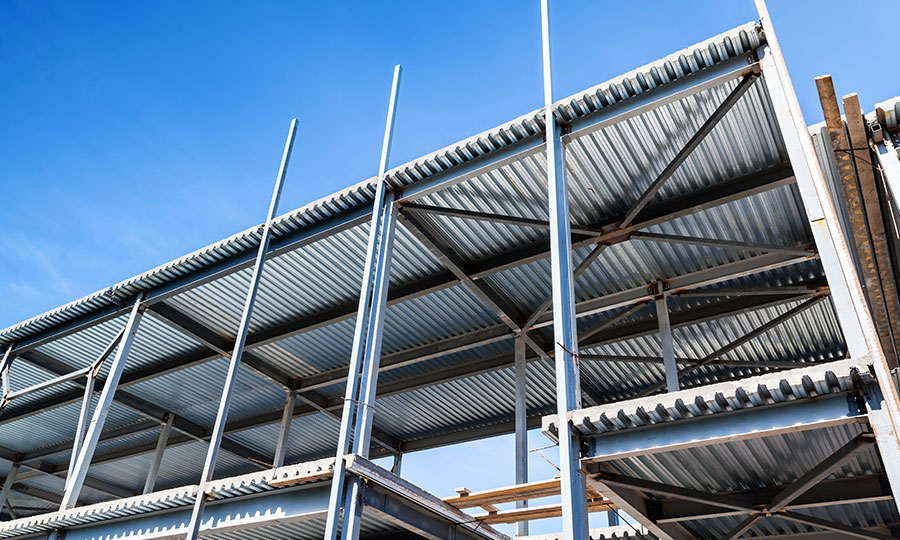
\includegraphics[width=0.7\textwidth]{losacero-1.jpg}
		\caption{sistema losacero PSI Concreto}
	\end{figure}
	
\begin{itemize}
	\item El sistema losacero ofrece seguridad, resistencia y varios beneficios para la construcción de edificaciones de distintos tipos.
	
	\item El perfil laminado de losacero está específicamente diseñado para quedar anclado con el concreto de manera precisa. Así se pueden formar las losas de azotea o entrepiso.
	
	\item El sistema losacero cuenta con estándares internacionales definidos principalmente por el Instituto Nacional Estadounidense de Estándares (ANSI) y el Steel Deck Institute (SDI).
	
	\item Este material está recomendado para instalaciones en las que se requiere de un soporte y seguridad bastante precisos, como los entrepisos y techos de hospitales, escuelas, estacionamientos y hoteles.
	
	\item Según el Steel Deck Institute, el losacero tiene tres funciones principales: actuar como plataforma de trabajo durante la construcción, proveer refuerzo positivo por flexión a la losa de concreto y otorgar resistencia para cargas horizontales.
\end{itemize}

		
	\subsubsection{Características generales}
	
	\begin{itemize}
		\item Las propiedades más importantes del sistema losacero se relacionan directamente con las ventajas que puede aportar a la construcción.
		
		\item Las láminas están hechas para sustituir a la cimbra tradicional de madera. De esta forma se puede pasar del colado a los acabados de forma directa.
		
		\item Las láminas son, por lo general, de acero galvanizado y cuentan con un diseño acanalado. Tienen un ancho de 91.5 centímetros (1), sobre el cual se coloca el concreto.
		
		\item Cuenta con conectores mecánicos, que aumentan la adherencia entre el concreto y el acero, con lo cual se evitan deslizamientos y se favorece el desempeño al ser una sola unidad o sistema.
		
		\item El concreto añadido actúa como un elemento de compresión para rellenar los canales hasta formar una superficie plana, en la cual se pueden realizar acabados a la losa.
		  \item Los decks metálicos son visibles en el techo de cada piso de la edificación.
		
		\item En PSI Concreto podemos asesorarte con tu proyecto de construcción y evaluar cuáles son tus mejores opciones de material para llevarlo a cabo. Haz clic para entrar en contacto con nosotros.
		
		\item El concreto es un material por excelencia para la construcción.
		Para conocer más, te invitamos a leer nuestra guía sobre las losas de concreto.
		
		
		
	\end{itemize}
	
	
	
	\begin{figure}[h]
		\centering
		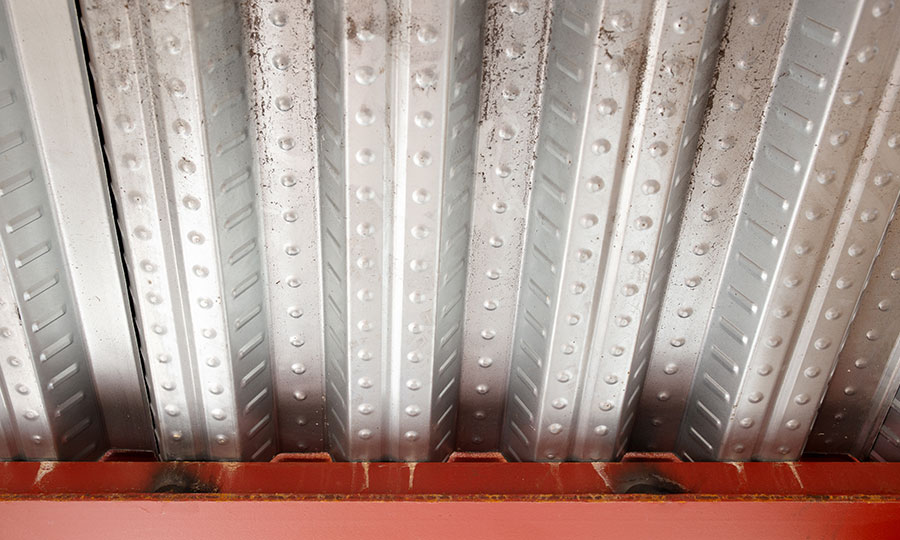
\includegraphics[width=0.7\textwidth]{losacero-2.jpg}
		\caption{decks metálicos PSI Concreto}
	\end{figure}

	
	
	\subsubsection{Beneficios del sistema losacero}
	
	\begin{itemize}
		\item Las ventajas del sistema losacero son bastante puntuales frente a otras alternativas de construcción y pesan mucho más que la desventaja principal que puede tener: un mayor costo que usar la típica cimbra de madera.
		
		\item El losacero es una opción altamente recomendada para zonas sísmicas, pues ofrece un buen nivel de seguridad por la manera en que funciona.
		
		\item Sin embargo, este mayor costo se ve atenuado con los otros beneficios que trae consigo. Entre ellos, destacan:
		
		\item Al funcionar como un sistema, permite que ante cualquier movimiento telúrico, las láminas, vigas y losas de concreto actúen en conjunto, previniendo el derrumbe de los techos.
		
		\item Su alta resistencia estructural le imprime durabilidad y, además, le brinda una buena protección ante condiciones ambientales, con viento, agua e incluso climas extremos.
		
		\item El hecho de que sustituya la cimbra de madera reduce el apuntalamiento temporal hasta en un 50\% (1).
		
		\item La eliminación de la cimbra de madera significa, además de un ahorro económico, una opción más ecológica, porque no se producen desechos de madera.
		
		\item El uso del acero propicia que distintos colados de azoteas y entrepisos se realicen al mismo tiempo, ya que forman una plataforma segura para continuar trabajando.
		
		\item Por lo anterior, se reducen de forma significativa los tiempos de construcción y, por ende, el costo de mano de obra.
		
		\item Es de fácil instalación y permite la disminución del número de apoyos de carga, por medio del incremento de espacios de separación.
		
		\item Todos estos beneficios hacen del losacero un sistema eficaz y seguro, además de adecuado para casi cualquier edificación. Recuerda consultar a especialistas de la construcción para obtener más información.
		
		\item Para cada tipo de construcción, hay distintos materiales. Haz clic para conocer los prefabricados de concreto, usados principalmente en carreteras y puentes.
	\end{itemize}
		
	
	
	\subsection{Componentes del losacero}
	
	Para entender mejor el funcionamiento y origen de las ventajas del sistema losacero, conviene conocer sus componentes:
	
	
	\subsubsection{Deck metálico}
	
	\begin{itemize}
	\item Los decks metálicos, de acero galvanizado, dotan de estructura y soporte firme a la edificación. Resisten los esfuerzos de tensión y tienen crestas con dentaciones que ayudan a fijar correctamente el concreto.
		
	\item Asimismo, cuentan con valles que, junto con las crestas, proporcionan mayor resistencia al cortante y permiten espaciar los apoyos metálicos. De hecho, las crestas y los valles distinguen a estos decks como específicos del sistema losacero.
	
	\item Los decks metálicos del losacero pueden llevar distintos acabados según se requiera, regularmente con fines decorativos.
	
	\end{itemize}
	
		
	\subsubsection{Acero de refuerzo y acero por temperatura}
	
	\begin{itemize}
	\item Cuando se requiere mayor durabilidad y seguridad, por ejemplo, en el caso de que el concreto y el metal no sean lo suficientemente resistentes por los esfuerzos en los extremos o al centro, se utiliza acero de refuerzo.
	
	
	\item Por lo regular, se agregan varillas, es decir barras de acero, en los apoyos y en el valle del deck metálico, según se determine. Si las varillas no absorben el cortante, entonces las placas y los perfiles de metal son otra opción.
	
	
	\item En caso de que el deck y el concreto absorban correctamente los esfuerzos, se suele agregar solamente acero por temperatura, por medio de varillas o malla electrosoldada.
	
	\end{itemize}
		
	
	\subsubsection{Pernos}
	
	
	\begin{itemize}
		
	\item Estos son los elementos de fijación para la instalación de los decks metálicos y el concreto en los puntos de apoyo. Los pernos tienen varias presentaciones y distintas alturas y diámetros.
	
	
	\item A las láminas de metal del sistema losacero pueden agregarse otros recubrimientos en su cara visible, especialmente con propósitos decorativos, como un galvanizado con pintura.
	
	
	\item Los pernos se colocan, por lo regular, en cada valle y apoyo, y así forman una retícula que distribuye la carga aplicada de manera directa sobre el concreto y hacia los puntos de apoyo.
	
	\item El otro material imprescindible es el concreto, que se coloca por encima del deck metálico y tiene que embonar perfectamente. Al concreto se le pueden realizar otros acabados y tratamientos.
	
	\item Para finalizar, sugerimos algunos aspectos importantes respecto a la instalación del losacero, como una guía de seguridad. No obstante, siempre es mejor realizar el trabajo de la mano de especialistas.
	
	
	\end{itemize}	

	
	\begin{figure}[H]
		\centering
		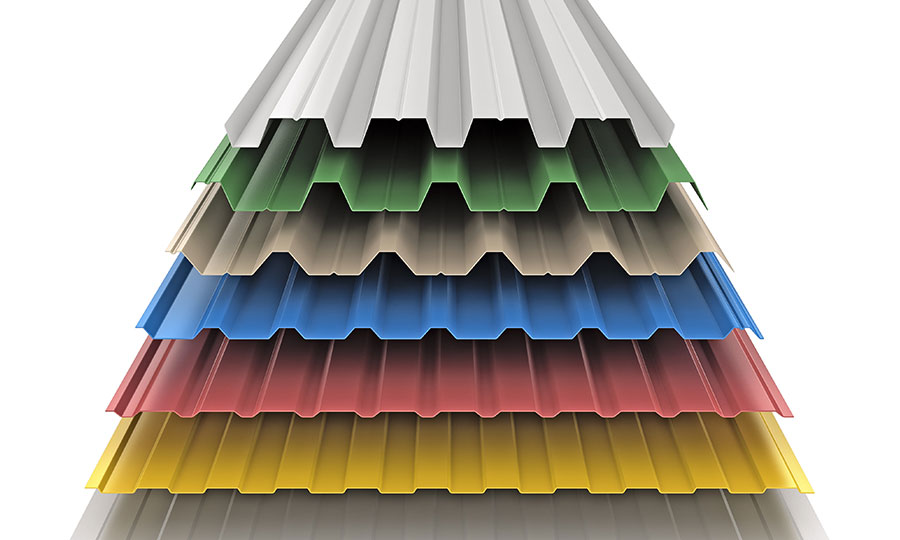
\includegraphics[width=0.7\textwidth]{losacero-4.jpg}
		\caption{acabados de los decks metálicos del losacero PSI Concreto}
	\end{figure}
	
	
	\subsection{Consideraciones para su instalación}
	
	Si bien hay que acudir con expertos para lograr un trabajo excelente, aquí te presentamos algunas sugerencias a la hora de la instalación:
	
	\begin{enumerate}
		
		\item Hay que cuidar una alineación muy precisa de los decks metálicos con los puntos de apoyo, para luego fijarlos con tornillos autotaladrantes o soldadura en cada valle.
		
		
		\item La soldadura y los tornillos autotaladrantes también serán útiles para fijar el traslape lateral de las láminas.
		
		
		\begin{figure}[h!]
			\centering
			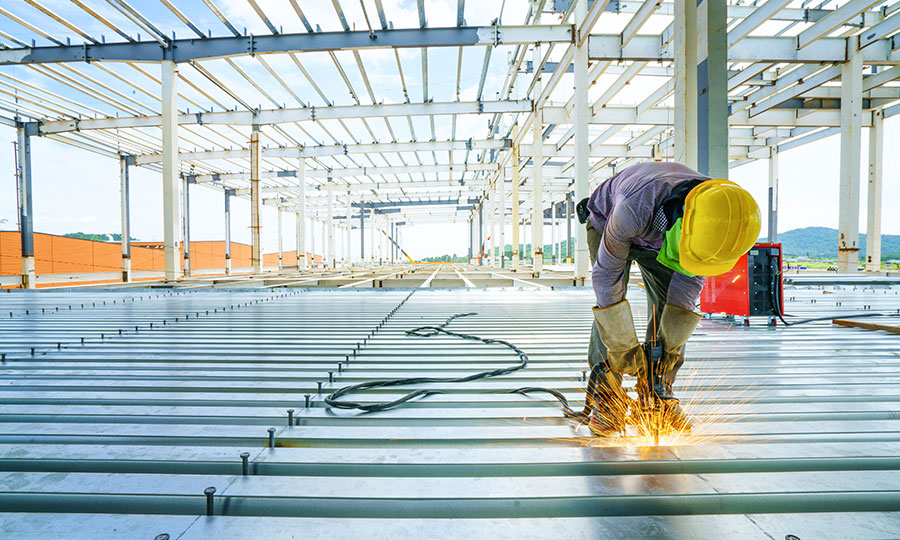
\includegraphics[width=0.7\textwidth]{losacero-3.jpg}
			\caption{instalación del losacero PSI Concreto}
		\end{figure}
		
		\item La soldadura es importante para el proceso de instalación del losacero. Esta es una de las técnicas que se usa para fijar las láminas o decks a los puntos de apoyo y entre ellas.
		
		
		\item Cuando se hayan instalado los decks, es tiempo de colocar la malla electrosoldada, es decir, el acero por temperatura. Se recomienda usar mallas en hojas precortadas para facilitar la aplicación.
		
		
		\item La colocación de tablas de madera para transitar sobre las láminas es una gran recomendación, así se evita la deformación de las crestas.
		
		
		\item El concreto debe ser colocado rápidamente de manera uniforme para evitar que se fragüe mientras está acumulado. En caso de bombearlo, la manguera deberá estar lo más baja posible para que no haya un impacto importante sobre el acero.
		
		
		\item Para las azoteas, es importante realizar un proceso de impermeabilización luego de haber colocado el sistema, con el objetivo de evitar que el agua se filtre fácilmente hasta el acero.
		
		
	\end{enumerate}
	
	\begin{itemize}
		
	\item Justamente la lluvia y la condensación por altos ciclos de temperatura generan humedad que, a su vez, puede corroer el metal del sistema. Es importante tener en cuenta esto tanto para las construcciones como para el almacenaje del losacero.
	
	
	\item Si tienes dudas sobre si el sistema losacero es ideal para tu construcción o quieres cotizar con el mejor precio y calidad, en PSI Concreto te atenderemos con gusto. Comencemos a colaborar juntos.
	
	
	\item El concreto ha ganado mucho terreno en la construcción de vías ferroviarias.Para saber más, lee nuestro artículo sobre durmientes de concreto.	
	
		
	\end{itemize}
	%-----------------------------------------------------








	
	%--------------SUBTITULOS 2---------------------
	
	% Segunda introducción
	\stepcounter{intro}
	\section*{\theintro\ Descripción y proceso constructivo de elementos de concreto}
	\addcontentsline{toc}{section}{\theintro\ Descripción y proceso constructivo de elementos de concreto}
	
	%REINICIAR CONTEO DE SECTION 
	\setcounter{section}{0}
		
	\section{Levantado de muros de Mampostería}
	El levantado de muros de mampostería es el proceso constructivo mediante el cual se construyen los muros de un edificio u obra utilizando unidades de mampostería (bloques de concreto, ladrillos de arcilla, piedra, entre otros) unidas con mortero.
	
	Así también consiste en disponer ordenadamente las unidades de mampostería en hiladas horizontales, siguiendo un trazo y plomo definidos, y asegurando que cada unidad quede ligada a las demás mediante mortero de pega. El levantado no se limita a “poner blocks”, sino que incluye la verificación de alineaciones, niveles, juntas llenas y continuidad estructural.
	
	\textbf{Características principales}:
	\begin{itemize}
		\item \textbf{Materiales}: bloques o ladrillos, mortero de pega y, en muchos casos, refuerzo (acero y graut).
		\item \textbf{Orden constructivo}: se inicia sobre la cimentación o sobre una solera de arranque, asegurando que la primera hilada quede perfectamente nivelada.
		\item \textbf{Juntas}: las horizontales y verticales deben quedar totalmente llenas de mortero para garantizar adherencia y estabilidad.
		\item \textbf{Refuerzo y confinamiento}: en sistemas sismorresistentes como los que regulan las NSE de Guatemala, el levantado incluye la previsión de columnetas, soleras y grauteo de celdas donde van alojadas las varillas.
	\end{itemize}
	
		\begin{figure}[h]
		\centering
		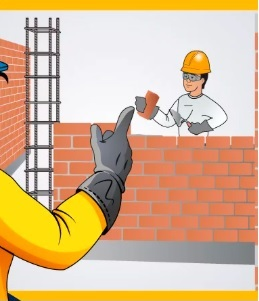
\includegraphics[width=0.4\textwidth]{mampos1}
		\caption{Muro de Mampostería}
		\end{figure}
	
	
		
	\subsection{Proceso constructivo}
	\subsubsection{Preparación y replanteo}
	\begin{enumerate}
		\item Revisión de planos y memorias conforme NSE 1 y NSE 7.4 (dimensiones, ubicación de columnetas/mochetas, soleras, vanos, cuantías). Registrar supervisión técnica.
		\item Cimentación y arranques listos (plomos de control). Nivelar y trazar ejes de muros y vanos.
		\item Unidades de mampostería (block/ladrillo) conformes a proyecto; verificar resistencia de unidades y f´m de la mampostería según tablas/criterios de la norma.
	\end{enumerate}
	
	\subsubsection{Mortero de pega}
	\begin{enumerate}
		\item Seleccionar tipo de mortero (p. ej. Tipo S o N, según exposición/cargas) y proporciones por desempeño conforme NTG 41050 (ASTM C270).
		\item Mezclado: materiales limpios, dosificación consistente; evitar exceso de agua.
		\item Controlar retención de agua y trabajabilidad (adherencia) según clima y succión de las unidades.
	\end{enumerate}
	
			
	\begin{figure}[h]
		\centering
		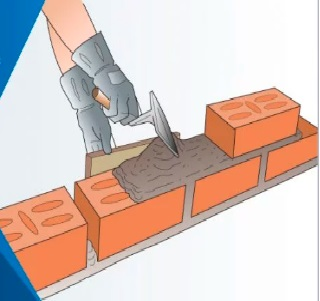
\includegraphics[width=0.4\textwidth]{mampos2}
		\caption{Distribución de mezcla}
	\end{figure}
		
	
	\subsubsection{Colocación de hiladas}
	\begin{enumerate}
		\item Primera hilada sobre mortero nivelado; controlar plomo, nivel y alineación.
		\item Espesor de juntas típico de 10 mm y llenado continuo.
		\item Minimizar el tiempo entre extender mortero y asentar la unidad (ideal $<$1 min) para no perder adhesión por succión/evaporación.
		\item Humedecido previo: si la unidad tiene alta succión, humedecer moderadamente; si es de muy baja succión, aumentar tiempo antes de asentar para evitar “flotación”.
	\end{enumerate}
	
		
	\begin{figure}[h]
		\centering
		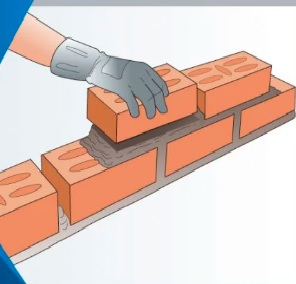
\includegraphics[width=0.4\textwidth]{mampos4}
		\caption{Colocación de ladrillo}
	\end{figure}
	
	
	
	\subsubsection{Armado y elementos de confinamiento}
	\begin{enumerate}
		\item Sistema confinado: muros con columnetas/mochetas y soleras de concreto que confinan el paño; es la modalidad prioritaria en Guatemala.
		\item Refuerzo en juntas de mortero no se reconoce con función estructural en la NSE 7.4.
		\item Columnetas: respetar límites de dimensiones y cuantías mínimas verticales ($\rho \geq 0.0075$, $\leq 0.02$) y mínimo 8 barras longitudinales con estribos adecuados.
		\item Dinteles y soleras: diseñar/armar según criterio de resistencia a corte y flexión, espaciamiento máximo de barras a flexión y, cuando aplique, refuerzo de corte; controlar deflexión y compatibilidad con la respuesta sísmica del marco/muro.
		\item Anclajes/pases: prever varillas, conectores, paso de instalaciones sin debilitar el diafragma del muro; coordinar con NSE-3.
	\end{enumerate}
	
	\subsubsection{Inyección (grauteo)}
	\begin{enumerate}
		\item Graut: elegir fino o grueso; convencional (asentamiento 200–280 mm) o autoconsolidante (flujo 610–760 mm; VSI $\leq$ 1), siempre con f’c $\geq$ 14 MPa a 28 días.
		\item Colocación por etapas: vibrado/varillado en graut convencional; continuidad entre levantados; no dejar “cuellos fríos”.
		\item Control de altura de levantado por jornada según especificación y práctica de obra.
	\end{enumerate}
	
	\subsubsection{Aperturas y remates}
	\begin{enumerate}
		\item Vanos con dinteles conformes a NSE 7.4; respetar apoyos mínimos, continuidad de soleras y confinamiento.
		\item Evitar concentrar instalaciones cerca de esquinas de vanos.
	\end{enumerate}
	
	\subsection{Curado y protección}
	\begin{itemize}
		\item Mortero (juntas): proteger del viento/sol para reducir evaporación; mantener humedad inicial suficiente (niebla ligera/pañete húmedo) sin encharcar.
		\item Graut: mantener condiciones que favorezcan hidratación; evitar lavado por lluvia; en autoconsolidantes, respetar recomendaciones del fabricante y NTG 41052.
		\item Clima:
		\begin{itemize}
			\item En calor/viento usar morteros con alta retención de agua.
			\item En frío llevar materiales $>$0°C antes de pegar, minimizar agua libre y proteger contra congelación.
		\end{itemize}
	\end{itemize}
	
	
		
	\begin{figure}[h]
		\centering
		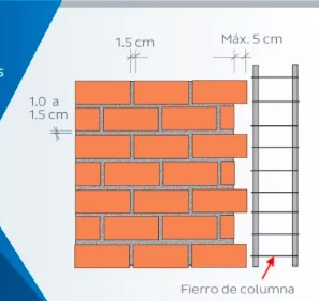
\includegraphics[width=0.4\textwidth]{mampos3}
		\caption{Espesor del mortero entre ladrillos }
	\end{figure}
	
	
	\subsection{Control de calidad y supervisión}
	\begin{itemize}
		\item Supervisión técnica obligatoria (NSE 1): bitácora, presencia en colocación de unidades, armaduras e inyección de graut.
		\item Materiales: verificar certificados de unidades, cemento, agregados; para graut usar NTG 41056 (ASTM C1019) para resistencia de compresión.
		\item Conformidad constructiva: la NSE 7.4 define propiedades geométricas (área neta/efectiva), colocación de lechos de mortero y no reconocer función estructural a varillas en juntas.
	\end{itemize}
	
	\subsection{Ventajas y desventajas}
	\subsubsection{Ventajas}
	\begin{itemize}
		\item Buen desempeño sísmico en vivienda de baja altura cuando se confinan paños y se respetan derivas/detalles (norma local específica).
		\item Disponibilidad de materiales y mano de obra en Guatemala; procesos conocidos.
		\item Rigidez lateral y compartimentación; facilidad para acabados.
		\item Compatibilidad normativa con NSE y referencia a TMS 402/602 para criterios puntuales.
	\end{itemize}
	
	\subsubsection{Desventajas}
	\begin{itemize}
		\item Sensibilidad a la calidad de ejecución (alineación, llenado de juntas y celdas, curado); errores reducen adherencia y capacidad.
		\item Interrupciones por vanos y mal resuelto de dinteles pueden crear debilidades locales si no se siguen los detalles de la NSE 7.4.
		\item Modificaciones posteriores (ranurados, pases) pueden comprometer el confinamiento si no se controlan.
		\item Peso propio mayor que sistemas livianos (implica considerar demanda sísmica conforme NSE-3).
	\end{itemize}
	%%-------------------------------------------------
	
	

	
	
	
	
	
	
	
	%%-------------MOCHETAS------------------------
	
	\section{Mochetas}
	
	La mocheta en mampostería es un elemento constructivo que forma un resalte o saliente en los muros de bloques o ladrillos, y que cumple funciones tanto estructurales como arquitectónicas.
	  
	Arquitectónicamente, se utiliza como acabado lateral de los vanos de puertas y ventanas, brindando mayor espesor y rigidez para recibir marcos, carpintería o cerramientos.  
	
	
	Estructuralmente, la mocheta puede actuar como jamba o elemento de confinamiento, mejorando la resistencia del muro frente a cargas verticales y laterales.  
	- En muchos casos, la mocheta se construye como parte de un sistema de mampostería reforzada, rellenando celdas de bloque con concreto y barras de acero, lo cual la convierte en un elemento capaz de resistir esfuerzos de compresión y cortante.  
	
	Según la NSE 7.4 de AGIES, las mochetas que funcionan como jambas de los vanos deben estar confinadas por soleras y castillos, además de contar con refuerzo vertical continuo. Esto asegura que, en caso de sismo, la apertura de vanos no debilite el muro.  
	 
	\begin{figure}[h]
		\centering
		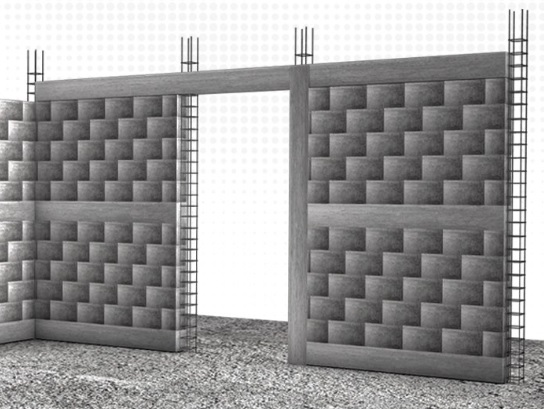
\includegraphics[width=0.6\textwidth]{mocheta1}
		\caption{Mocheta en mampostería reforzada}
	\end{figure}

	
	\subsection{Proceso constructivo de mochetas en mampostería}
	
	\subsubsection{Preparación y replanteo}
	Se trazan en obra las dimensiones de la mocheta, que normalmente coincide con el espesor del muro y un ancho de 10 a 30 cm. Se marcan las ubicaciones de refuerzos verticales, que deben alinearse con cimentaciones y soleras superiores. Se verifican los niveles y plomos para evitar desviaciones.  
	
	\subsubsection{Armado y refuerzo}
	Se colocan barras longitudinales en las celdas de bloque que formarán la mocheta.  
	- Para mochetas pequeñas: Ø 3/8” (\#3).  
	- Para mochetas de jamba: Ø 1/2” (\#4) o superior, dependiendo del cálculo.  
	El refuerzo debe anclarse en la cimentación y tener traslapo en la solera superior. Se recomienda usar amarres transversales o ganchos a 90° para integrarse mejor con el muro.  
	
	
	\subsubsection{Levantado de la mocheta}
	Se colocan bloques o ladrillos de forma alternada, cuidando la trabazón con el muro. En cada 40–60 cm de altura, se alinean las juntas verticales con las barras de acero. Las celdas con acero se rellenan con concreto fluido de  $f'_{c} \geq 210 \,\text{kg/cm}^2$, recomendado por la NSE 7.4. Se vibra o varilla el relleno para evitar vacíos.  
	
	\begin{figure}[h]
		\centering
		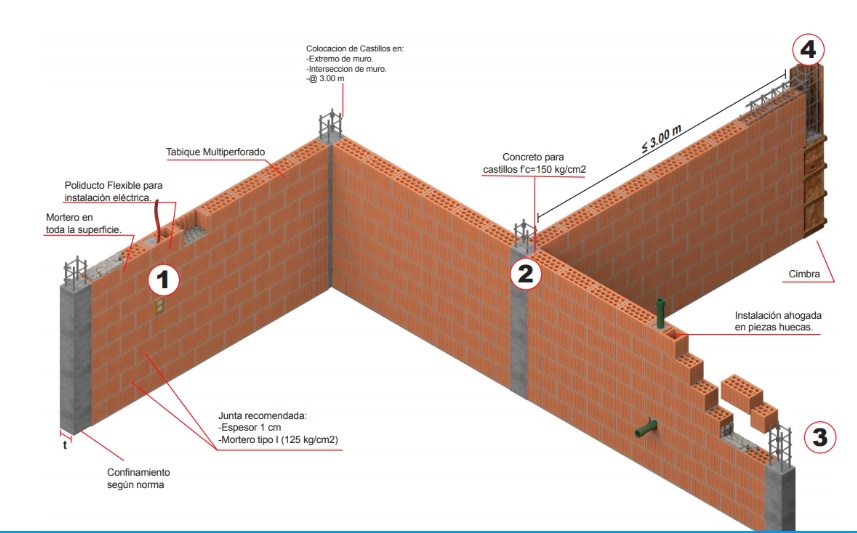
\includegraphics[width=0.6\textwidth]{mocheta3}
		\caption{Distribución de mochetas}
	\end{figure}
	
	\subsubsection{Instalación de soleras y confinamiento}
	Una vez alcanzada la altura del vano o techo, se coloca una solera de concreto armado, que amarra la mocheta con el muro. Si la mocheta está junto a un vano, se conecta con el dintel, formando un marco de confinamiento.  
	
	\subsubsection{Curado}
	El mortero de pega debe mantenerse húmedo al menos durante 3 días, cubriéndose con plásticos o regando periódicamente.  
	El concreto colado en las celdas y soleras debe curarse según ACI 308R:  
	- Mantenerlo húmedo durante 7 días.  
	- En climas cálidos y secos (ej. oriente de Guatemala), usar membranas de curado para evitar evaporación rápida.  
	- En el altiplano frío (ej. Quetzaltenango), controlar el curado para evitar fisuración por baja temperatura nocturna.  
	
	\subsection{Instalación y coordinación}
	Las mochetas deben levantarse de forma solidaria al muro, asegurando que no queden juntas frías. Se deben prever ductos o cajas eléctricas dentro de la mocheta si pasan instalaciones. Se controla la verticalidad y el aplome en cada hilada. En proyectos sismo-resistentes, las mochetas deben estar amarradas a la estructura principal mediante soleras, castillos y refuerzos continuos.  
	
	\subsection{Ventajas y desventajas}
	
	\subsubsection{Ventajas}
	- \textbf{Resistencia}: incrementan la capacidad portante del muro.  
	- \textbf{Confinamiento sísmico}: según NSE 7.4, mejoran el comportamiento ante cargas laterales.  
	- \textbf{Integración arquitectónica}: sirven como acabado de vanos, ocultando imperfecciones.  
	- \textbf{Durabilidad}: con buen curado y protección, son altamente resistentes al desgaste.  
	- \textbf{Versatilidad}: se adaptan a diferentes anchos y materiales de mampostería.  
	
	\subsubsection{Desventajas}
	- \textbf{Costo adicional}: requieren acero, concreto y mano de obra calificada.  
	- \textbf{Tiempo de ejecución}: demanda mayor planificación que un muro simple.  
	- \textbf{Fisuración}: si no se curan correctamente, aparecen grietas longitudinales.  
	- \textbf{Rigidez excesiva}: pueden generar concentraciones de esfuerzos si no están bien integradas al muro.  
	- \textbf{Limitación en remodelaciones}: dificultan hacer nuevas aberturas.  
	
	  
	
	
	
	
			

\end{document}
